
\documentclass[runningheads]{llncs}

\usepackage{graphicx}
\usepackage{float}
\usepackage{amsbsy}
\usepackage{tabularx}
\usepackage{bbm}
\usepackage{float}
\usepackage[english]{babel}
\usepackage[utf8]{inputenc}
\usepackage{amsmath}
\usepackage{amsfonts}
\usepackage{algorithm}
\usepackage{algpseudocode}
\usepackage{graphicx}
\usepackage{mwe}
\usepackage{dsfont}
\usepackage{subcaption}
\usepackage{caption} 
\captionsetup[table]{skip=10pt}
% \renewcommand\UrlFont{\color{blue}\rmfamily}

\begin{document}

\title{Emotion detection in song lyrics}


\author{Simone Quadrelli}

\institute{Università Statale degli studi di Milano,
\email{simone.quadrelli@studenti.unimi.it}}

\maketitle            

\section{Introduction}
The hereby paper addresses the challenge of detecting emotions and their intensity from the text of tweets via machine learning and aims to transfer the prediction capabilities to predict songs emotions and their intensity from the lyrics. These information allows to fathom the existence of correlations between musical genres and sentiments and between authors and sentiments.\\

Emotion detection has a widespread applications in many fields: it is used in marketing to tune and evaluate advertisement, it is exploited to monitor elections and the preference of voters and it is part of music recommendation systems in many streaming applications. 
Despite emotion detection being increasingly used in many field, still some remarkable issues remain. There is disagreement about the way sentiment should be measured: some suggest to use valence, arousal, and dominance features, others prefer to use simple categorical variables. Moreover, there are few reliable datasets for emotion detection in song lyrics and just some of them have a suitable dimension for supervised learning. Indeed, a very small dataset, consisting in less than two hundred songs has been constructed by R. Malheiro et al. in \cite{musicmood}. Another issues concerns the emotions to be used: if the number of emotions (or moods) is too big then the subjectivity of annotators may be too much and they should be clustered into wider emotions, if just positive or negative moods are involved, as in \cite{musicmood1}, they may be too few to be significant. In the end, for music recommendation systems using just lyrics may not be enough and the melody should be equally taken into account. \\



\section{Research question and methodology}
The objective of this work is two-fold: to develop predictors of sentiment and intensity and to study whether or not there exist a correlation between genre and sentiments in song lyrics. Achieving this objectives is not straightforward and requires to transfer the prediction capability of predictors trained on labelled twits to unlabelled songs. Moreover, for the delight of the user, it is possible to create a playlist given a chosen genre and sentiment. \\

Formally, the first objective consists in finding a transform $\phi: \mathcal{D} \rightarrow \mathcal{F}$ to map documents into numerical features suitable for machine learning. Then it is required to select the best classifier $h: \mathcal{F} \rightarrow \mathcal{Y}$ that maps the features $\mathcal{F}$ into sentiments $\mathcal{Y}$ and the best predictor for intensity $h^{\prime}: \mathcal{F} \rightarrow \mathcal{I}$ that maps features into intensity $\mathcal{I}$.  Then exploiting the features extracted from the song lyrics via $\phi$ it is possible to use $h$ and $h^{\prime}$ to assign sentiment and intensity to songs. \\
In the end, the correlation between the unconditional distribution of the sentiment and conditional distribution of the sentiment given the genre, is tested by $\chi^2$ test.

To clarify the overall description of the process that leads to the computation of the correlations and the creation of playlists the reader may refer to Figure \ref{fig:schema}.
\begin{figure}[H]
    \centering
    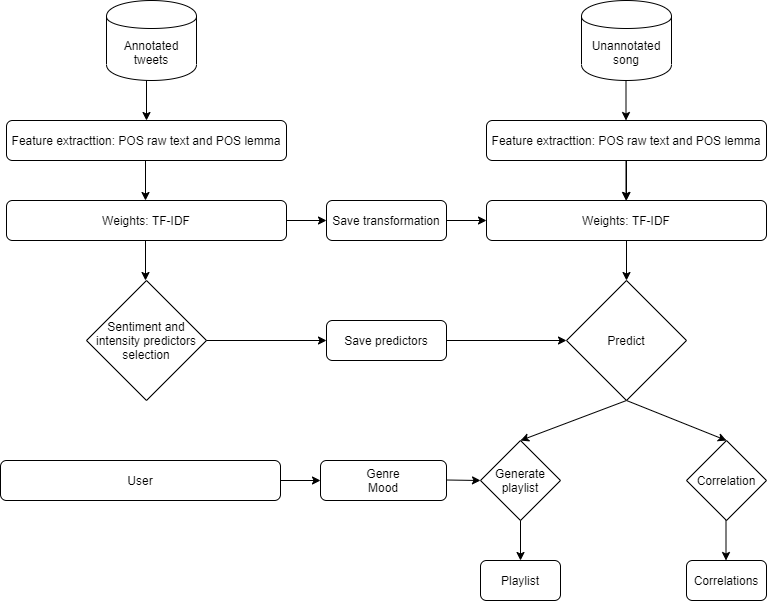
\includegraphics[width=1\textwidth]{images/schema.png}
    \caption{Schema of the project}
    \label{fig:schema}
\end{figure}
A more in-depth description of the process along with some experiments and their results will be detailed in the following section.\\

\section{Experimental results}
As stated before, two datasets are involved in the analysis: one containing 3613 tweets\footnote{https://saifmohammad.com/WebPages/EmotionIntensity-SharedTask.html} and the other one concerning 362237 songs form MetroLyrics\footnote{https://www.kaggle.com/gyani95/380000-lyrics-from-metrolyrics}. The dataset of tweets is composed by three variables: text, sentiment and intensity, where labels in sentiment belongs to the set \{anger, fear, joy, sadness\} and intensity $\in [0,1]$. The song dataset contains the variable: title, lyrics, year, artist and genre. \\

Among all the possible metric to evaluate the performance of classifiers F1-score $\in [0,1]$ seems a suitable choice:
\begin{equation}
    \text{F1-score} = 2 \cdot  \frac{precision \cdot   recall}{precision + recall}.
\end{equation}
It is the armonic mean of precision ($precision = \frac{tp}{tp+fp}$) and recall ($recall = \frac{tp}{tp+fn}$), which can be defined starting from the notions of true positive ($tp$), false positives ($fp$) and false negative ($fn$).
Since there are four labels and F1-score works just for binary labels, it is computed class-wise and then scores are averaged.\\

For the intensity estimation, a suitable measure is the mean absolute error (MAE) between the predicted intensity $\hat{y}$ and the ground truth $y$ computed on $N$ predictions as
\begin{equation}
    \text{MAE}(y,\hat{y}) = \frac{1}{N} \sum_{i=1}^N |y_i-\hat{y}_i|
\end{equation}
\\

Bearing in mind the descriptions of the datasets and the knowledge of the metrics it is possible to dig deeper into the analysis descirbed in Figure \ref{fig:schema}.\\
The very first preprocessing step to clean the corpus consists in removing punctuation and other sequence of characters that carry no information, for instance, the various new line symbols in song lyrics. Even after this preliminary step, it is possible to manipulate the documents in the corpus to map similar words into the same basic expression that must be a word of the vocabulary. This process is known as lemmatization and the basic expressions retrieved are called lemmas. Even if lemmas are extracted, a lot of useless information remains, for instance: pronouns, articles and very frequent verbs. It is possible to select only some interesting part of speech (POS) elements such as nouns and adjective to use what are expected to be very informative words or lemmas. At the end of this first processing nouns and adjective both in lemmatized and not lemmatized form were selected, since they are more likely to convey emotional information. To be able to train classifiers data should be converted into some suitable numerical form by $\phi$. To overcome the issue, it is possible to use Term frequency - inverse document frequency schema to give higher weights to presumably more important words.
This weighting schema can be applied when the data have been vectorized. Indeed it is possible to embed the text into a numeric matrix $M_{N \times W}$, where $N = |D|$ is the number of documents in the corpus $D$ and $W$ is the total number of unique words (or lemmas) in it.
The term frequency $ft(t,d)$ of a terms $t$ in a document $d$ is 
\begin{equation}
    tf(t,d) = \frac{f(t,d)}{\sum_{t^{\prime} \in d}f_{t^{\prime},d}},
\end{equation}
where $tf(t,d) = \mathds{1}\{t \in d\}$.

The inverse document frequency $idf(t,D)$ is the logarithm of the ratio between the total number of documents and the number of time the term $t$ appears in the set of documents $D$
\begin{equation}
    idf(t,D) = \log \biggl ( \frac{N}{\sum_{d=1}^{D} \mathds{1}\{t \in d\}} \biggr )
\end{equation}

From this two quantities it is possible to obtain tf-idf weights as
\begin{equation}
    \text{tf-idf}(t,d,D) = tf(t,d) \cdot idf(t,D)
\end{equation}
After the weights have been computed the python object that computes the transformation is saved to be later used to extract the weights from song lyrics. \\

Before proceeding to the model selection, there is issues tackle: the dataset is unbalanced; indeed, the class fear has higher frequency than the other ones. To prevent classifiers from predicting too many instances of class fear, an oversample procedure is applied. Hence, the final dataset is perfectly balanced. \\
There is also choice to make when deciding how to handle the prediction task: either train predictors that output sentiment and intensity together or a  classifier for the sentiment and an independent predictor for the intensity. Since the correlation between sentiment and emotion, computed by Spearman's correlation test, is very close to zero, the latter approach seems a valid and much simpler option. Hence, there two different problems arise: it is necessary to select the best classification model for the sentiment and the best regression model for the intensity. For classification, the best model was selected accordingly to the cross-validated F1-score among K-nearest neighbours (KNN), random forests (RF) and SVMs. Analogously the best regression model was selected accordingly to the cross-validated mean absolute error among the previous classes modified for regression models. This procedure is performed two times using as features POS lemma and POS raw text. 

\begin{table}[H]
    \caption{Performance of predictors}
        \label{tab:models}
    \begin{subtable}{.5\linewidth}
      \centering
        \caption{Classification performance}
        \begin{tabular}{||c |c |c||} 
 \hline
 Predictor & Features & F1-score \\ [0.5ex] 
 \hline\hline
 KNN & POS lemma & 0.66  \\ 
 \hline
 KNN & POS raw & 0.61  \\ 
 \hline
 RF & POS lemma & 0.70  \\ 
 \hline
 RF & POS raw & 0.70  \\ 
 \hline
 SVM & POS lemma & 0.87  \\ 
 \hline
 SVM & POS raw & 0.89  \\ 
 \hline
\end{tabular}
    \end{subtable}%
    \begin{subtable}{.5\linewidth}
      \centering
        \caption{Regression performance}
       \begin{tabular}{||c |c |c||} 
 \hline
 Predictor & Features & MAE \\ [0.5ex] 
 \hline\hline
 KNN & POS lemma & 0.14  \\ 
 \hline
 KNN & POS raw & 0.14  \\ 
 \hline
 RF & POS lemma & 0.15  \\ 
 \hline
 RF & POS raw & 0.15  \\ 
 \hline
 SVM & POS lemma & 0.11  \\ 
 \hline
 SVM & POS raw & 0.11  \\ 
 \hline
\end{tabular}
    \end{subtable} 
\end{table}

As can be seen from Table \ref{tab:models}, the best models for sentiment and intensity is the SVM for classification and the SVM for regression with POS raw text features and indeed they are applied to songs to assign them sentiment and intensity. Then the intensity is used to select the songs that have at least intensity higher that $0.5$, assuming that if the intensity is too low, then the predicted sentiment may not be relevant. \\

As previously stated, one objective of this work is to understand whether or not there is a correlation between genre and sentiment. In order to understand it is possible to run the $\chi^2$ test for independence between the unconditional distribution of sentiment (see Table \ref{tab:sentimentdistribution}) and the distribution of sentiment within each class (see Figure \ref{fig:correlations}). 

\begin{table}[H]
    \centering
    \begin{tabular}{|c |c |c|c|} 
     \hline
     Anger & Joy & Fear  & Sadness\\ [0.5ex] 
     \hline
     0.17 & 0.32 & 0.26  & 0.25 \\ 
     \hline
    \end{tabular}
     \caption{Unconditional distribution of the sentiments}
    \label{tab:sentimentdistribution}
\end{table}



As Figure \ref{fig:chi_square} shows, there is correlation between sentiments and genres, indeed the p-values are 0 and the test scores are remarkably high and therefore the independence hypothesis should be rejected.
\begin{figure}[H]
    \centering
    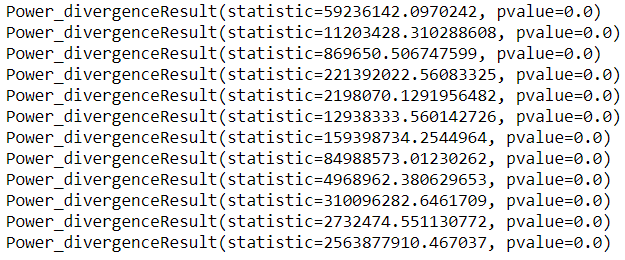
\includegraphics[width=0.95\textwidth]{images/chi_squared.PNG}
    \caption{$\chi^2$ test results}
    \label{fig:chi_square}
\end{figure}
Moreover, from the confusion matrix (see Figure \ref{fig:correlations}) of genres and sentiment, normalized by columns, it is possible to appreciate the difference in the distribution of sentiments in each genre.
\begin{figure}[H]
    \centering
    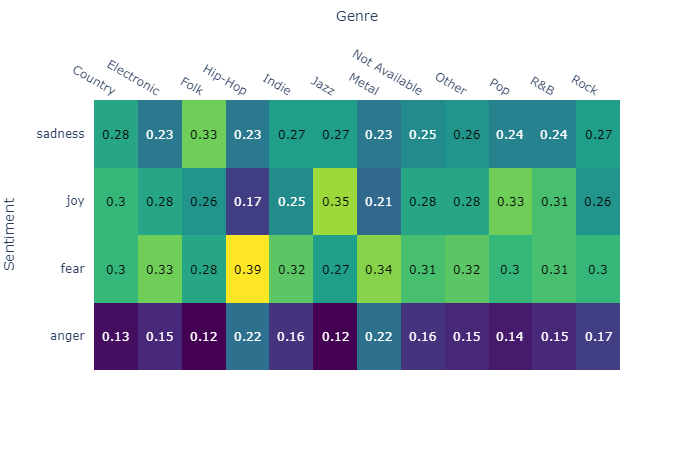
\includegraphics[width=0.95\textwidth]{images/correlation.png}
    \caption{Correlation between genre and sentiment of songs whose intensity is greater than 0.5}
    \label{fig:correlations}
\end{figure}

It is also possible to analyze the sentiment of different authors for which a relevant number of songs is present as Figure \ref{fig:artists} shows.
\begin{figure}[H]
    \centering
    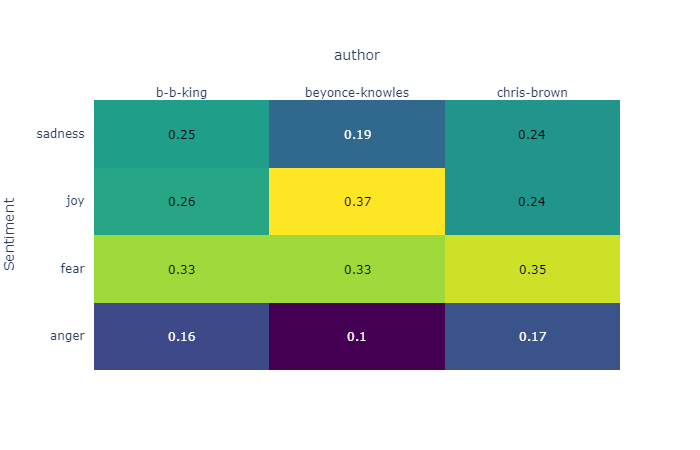
\includegraphics[width=0.95\textwidth]{images/artists.png}
    \caption{BB King's, Beyoncé's, Chris Brown's songs sentiments}
    \label{fig:artists}
\end{figure}
Moreover, given the genre and the sentiment provided by the user, the software outputs a personalized playlist. It is computed in two steps: first songs of the specified genre and sentiment are selected and then they are sorted by intensity: Figure \ref{fig:playlist} provides some example of playlists generated by the software.

\begin{figure}
     \centering
     \caption{Example of playlists}
     \label{fig:playlist}
       \hfill
     \begin{subfigure}[b]{0.4\textwidth}
         \centering
         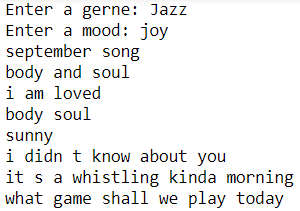
\includegraphics[width=\textwidth]{images/jazz_joy.PNG}
         \caption{Playlist containing the most intense jazz song with respect to joy}
         \label{fig:y equals x}
     \end{subfigure}
     \hfill
     \begin{subfigure}[b]{0.4\textwidth}
         \centering
         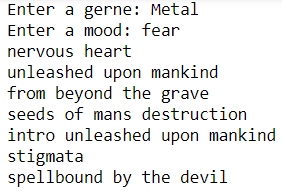
\includegraphics[width=\textwidth]{images/metal_fear.PNG}
         \caption{Playlist containing the most intense metal song with respect to fear}
         \label{fig:three sin x}
     \end{subfigure}
     \hfill
\end{figure}

\section{Concluding remarks}
Overall, there is a correlation between genre and sentiments as the $\chi^2$ tests clearly show (see Figure \ref{fig:chi_square}). Anger is the less frequent sentiment, even if the frequency of joy, sadness and anger is very similar in the original unbalanced dataset. On the contrary, the great amount of fear labels may come from the dataset which was originally unbalanced. The oversample procedure is such that some example of the less frequent sentiments are repeated but it may not be enough to completely remove the bias that comes from the original unbalancedness. Moreover, there are some interesting findings: a remarkable amount hip-hop and metal songs are labelled with fear but I would expect metal to be more related to anger while hip-hop to joy. On the contrary, jazz songs are strongly connected to joy and this seems a sound result. It is also worth noting that folk is the only genre whose songs are most frequently labelled with sadness.\\ 
The sentiment distribution of Beyoncé is very peculiar: indeed it has a very low number of anger labels and joy is remarkably high, even more if compared to pop sentiment distribution (see Figure \ref{fig:artists}). B.B. King, a jazz guitarist, has a distribution skewed toward fear, while the most frequent sentiment in jazz songs is joy (see Figure \ref{fig:artists}). \\
A last remark, even if the title may convey useful information about the sentiment it was not used as feature so that it can be exploited by the reader as an independent test to assess the precision of the model.\\

However, songs should not be categorized by the text alone, the music is at least as important as the lyrics. An interesting possibility is to analyze the music of these song to better predict the sentiment. Another possible future work may be consist in comparing the results of this work with those from an annotated and comparable dataset of song lyrics.\\

\begin{thebibliography}{8}

\bibitem{musicmood}
R. Malheiro, R. Panda, P. Gomes  R. Paiva. Emotionally-relevant features for classification and regression of music lyrics. In: IEEE transactions on affective computing, (2016).

\bibitem{musicmood1}
S. Raschka. MusicMood: Predicting the mood of music from song lyrics using machine learning. (2016).
\end{thebibliography}

\end{document}